%% --------------------------------------------------------------
%% Imitation Learning applied to predictive maintenance
%%
%% V.1.0: Re-baselined. 17-Sep-2024
%%
%% --------------------------------------------------------------

\documentclass{article}
\usepackage[top=2in, left=1.5in,right=1in,bottom=1in]{geometry} 
\usepackage[style=authoryear, backend=bibtex, natbib]{biblatex}

\usepackage{graphicx}
\usepackage{floatrow}

\addbibresource{bibliography.bib} % Bibliography file
\usepackage[hidelinks]{hyperref}	% links
\hypersetup{colorlinks = true, urlcolor = blue, linkcolor = blue, citecolor = blue}
\usepackage{xcolor, soul} 	% Highlights
\usepackage{booktabs}		% Tables
\usepackage{array}			% Tables with word-wrap
\usepackage{ragged2e}		% Ragged edges in tables
\usepackage{arydshln} 		% dashed lines in tables
\usepackage{setspace}
\usepackage{multirow}
\usepackage{amsmath}
\usepackage{algorithm}
\usepackage{algpseudocode}

\newfloatcommand{capbtabbox}{table}[][\FBwidth] % Bottom caption, box width adjusted to content

\onehalfspacing

%%% MACROS
\newcolumntype{L}[1]{>{\raggedright\arraybackslash}p{#1}}
\newcolumntype{R}[1]{>{\raggedleft\arraybackslash}p{#1}}
\newcommand{\hlc}[2][blue!10]{{\colorlet{foo}{#1} \sethlcolor{foo}\hl{#2}}}
\algnewcommand{\Inputs}[1]{%
	\State \textbf{Inputs:}
	\Statex \hspace*{\algorithmicindent}\parbox[t]{.8\linewidth}{\raggedright #1}
}
\algnewcommand{\Initialize}[1]{%
	\State \textbf{Initialize:} {\raggedright #1}
	% \Statex \hspace*{\algorithmicindent}\parbox[t]{.8\linewidth}{\raggedright #1}
}

%opening

%\title{Beyond Reinforcement Learning: A Tutorial on Applying Reward Learning to Predictive Maintenance}
%\title{Beyond Reinforcement Learning: Learning to Imitate the Predictive Maintenance Engineer}
\title{Beyond Reinforcement Learning: Learning to Imitate the Expert Predictive Maintenance Engineer.\\\textcolor{red}{\small{V.1.0}}}
\author{Rajesh Siraskar}

\begin{document}
\maketitle
\begin{abstract}
	Most developed countries are facing a crisis. An ever increasing proportion of expert work force retiring combined with fewer workers. This threatens the economic growth of industrialized countries, like Germany. This article is a short survey and tutorial on applying Behavioral Cloning, an artificial intelligence algorithm that learns to imitate an expert. We show how it can be applied to the domain of industrial predictive maintenance. The role of the maintenance engineer in ensuring the smooth, disruption free, running of industrial machines is indispensable. Industrial plants depend on the expert judgment of the maintenance engineer to estimate machine part failures just so much in advance that quality of product is not affected and yet not so much in advance that the part's effective useful life is not fully utilized. While human judgment is undeniably superior to computer based algorithmic systems, they cannot physically cater to hundreds of machine parts simultaneously. Advances in reinforcement learning technology have enabled autonomous predictive maintenance of large scale plants. These algorithms replicate the human learning mechanism and optimize the part replacement problem using "cost functions". Design of reinforcement learning cost functions remains a "hand crafted" process. This article explores the application of Learning from Demonstration applied to this task for the predictive maintenance. This paper first provides a basic understanding of \hlc{IRL, inverse reinforcement learning}. We study broadly where it has been applied, emphasizing their applicability to the predictive maintenance domain. Using expert examples of desired tool replacement patterns the "Imitation Learning" learns human like replacement patterns. In the form of a tutorial, this paper demonstrates an implementation of the Behavior Cloning algorithm. We use the standard benchmark \hlc{IEEE PHM 2010} dataset and present experimental results.
\end{abstract}

\clearpage
\section{APPROACH}
\begin{enumerate}
	\item Tech background: First finish STANFORD
	\item \quad BC - only - max Dagger - rest say beyond scope
	\item Survey! === Sec.\ref{sec:SLR}
	\item \quad Taxonomy --- Stanford lec + OSA + 1 survey is enough === Sec.\ref{sec:Taxonomy}
	\item Tutorial! === Sec.\ref{sec:Tutorial}
\end{enumerate}
\subsection{IMPORTANT REFS}
\begin{enumerate}
	\item business refs:
	Right now, one-quarter of the manufacturing workforce is over 55 years old. Meanwhile, the manufacturing industry is struggling to attract enough younger workers with the right skills and qualifications.  \href{https://fortune.com/europe/2024/05/29/germany-aging-population-economy-europe-growth-productivity-workforce-imf/}{Fortune}\href{https://www.imf.org/en/News/Articles/2024/03/27/germanys-real-challenges-are-aging-underinvestment-and-too-much-red-tape}{IMF}; 
	\item \href{https://web.stanford.edu/class/cs237b/pdfs/lecture/cs237b_lecture_12.pdf}{Stanford lecture} -- 14 pgs - SOLID foundation - use to sort out terms:
	\begin{itemize}
		\item Inverse Reinforcement Learning  
		\item Apprenticeship Learning 
		\item Maximum Margin Planning
		\item Maximum Entropy Inverse Reinforcement Learning
		\item Learning From Comparisons and Physical Feedback
	\end{itemize}
	\item \cite{Osa-2018} - Algorithmic Perspective on IL - see images/illustrations etc.
	\begin{enumerate}
		\item \hlc{TAXONOMY} - add Model-based/Model-free and more
		\item Pg. 17, Sec. 1.3 
		\hlc{Key Differences between Imitation Learning and Supervised Learning} -- "For example, when transferring human skills to a humanoid robot, the motion captured from a human expert may be infeasible for the humanoid. In such a case, the demonstrated motion needs to be adapted to be feasible for the humanoid. This kind
		of adaptation is less common in the standard supervised learning"
		\item In imitation
		learning, the demonstration dataset does not cover all possible
		situations since collecting expert demonstrations to cover all situations
		is usually too expensive and time-consuming. As a result, the learner
		often encounters states which were not encountered by the expert during
		demonstrations, which means that the target domain distribution is
		different from the source distribution. Therefore, covariate shift or domain
		adaptation is closely related to imitation learning [Bagnell, 2015].
		\item \hlc {prior knowledge that allows for dramatically more efficient methods. Recent work by} \cite{sun2017} \hlc{demonstrates a potentially exponential decrease in sample complexity in learning a task by imitation rather than by trial-and-error reinforcement learning, and
			empirical results have long shown such benefits} \cite{abbeel2010autonomous} [Silver et al., 2016, Kober and Peters, 2009, Abbeel et al., 2010].
	\end{enumerate}
	\item \href{https://underactuated.mit.edu/imitation.html#:~:text=Broadly%20speaking%2C%20most%20approaches%20to,the%20data%20using%20supervised%20learning.}{Russ Tedrake MIT lecture \citep{TedrakeLecture2023}} - \hlc{USE \textbf{ONLY} for this quote and cite. Else } -- ``BC is interesting! used from LLM OPEN AI to the shortest path to building `robot foundation models`"  and for the opening para "Broadly speaking, most approaches to imitation learning can be categorized as either behavior cloning (BC) or inverse reinforcement learning (IRL). Behavior cloning attempts to learn a policy directly from the data using supervised learning. Inverse RL (aka inverse optimal control) attempts to learn a cost function from the data, and then uses potentially more traditional optimal control approaches to synthesize a policy for this cost function, in the hopes of generalizing significantly beyond the demonstration data"
	\item \href{https://ai.stanford.edu/~ang/papers/icml04-apprentice.pdf}{Apprenticeship Learning via Inverse Reinforcement Learning}
\end{enumerate}
\begin{enumerate}
	\item \cite{torabi2018BCO} -- BC from observation only: Possibly in the ``future direction'' section: [This is already my words] While BC provided a good introduction to imitation learning and is a simple algorithm, \cite{torabi2018BCO} provides an interesting algorithm, named BCO($\alpha$), that allows quick learning from observations \textit{only} (i.e., \textit{without} explicit action information. This is achieved using a two-step process.
\end{enumerate}
\clearpage
\section{Introduction}

\textcolor{blue}{Most developed countries are facing a crisis. According to the IMF and Fortune, an ever increasing proportion of expert work force retiring combined with fewer workers}, \citep{Prakash2024Germanys, Fletcher2024Germanys}. \textcolor{red}{Right now, one-quarter of the manufacturing workforce is over 55 years old. Meanwhile, the manufacturing industry is struggling to attract enough younger workers with the right skills and qualifications.} \href{https://nam.org/new-report-dives-into-retaining-the-aging-manufacturing-workforce-5579/?stream=workforce}{nam.org}

Reinforcement Learning (RL) is a machine learning technique that mimics the trial-and-error learning mechanism humans and animals use to learn a new task. A 'task' is a 'problem' such as learning to play chess, or for a robot painting, assembling automotive components is a task. The task we will focus on will be ``predictive maintenance''. The core elements of RL are shown in Figure \ref{fig:RL}.
\begin{figure}[h]
	\centering
	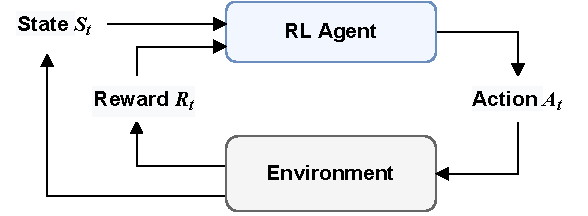
\includegraphics[width=0.5\linewidth]{images/RL-loop.pdf}
	\caption{The Reinforcement Learning mechanism.}
	\label{fig:RL}
\end{figure}

The `agent' is the learner. It learns by continuously interacting with its \textit{environment} and gathering feedback for every action $A_t$ it takes. When an action ($a\in \mathcal{A}$) is performed, the environment changes from an existing `state' $S_t$ and presents a new `state' $S_{t+1}$. A state ($s\in \mathcal{S}$) represents a specific condition of the modeled environment or system and is designed to contain all the relevant information needed by the agent to make decisions to achieve the objective. This state could be classified as being `good' or `bad' for the learning objective. For example, consider learning to ride a bicycle where moving forward is desirable, whereas falling isn't. Similarly, for predictive maintenance, successfully completing a maintenance task and ensuring a longer life of equipment is a positive outcome, whereas premature failure of equipment isn't. As in humans, the objective of learning a task is achieved when the actions that generate the favorable state are mastered. RL uses rewards (or penalties) to reinforce good behavior over bad. Rewards $R_{t+1}$ are scalar values that serve as the feedback signal. Over time, the agent attempts to maximize (or minimize) the rewards, and this reinforces good actions over bad, enabling it to learn an optimal `policy'. A policy $\pi$ is a mapping from states to probability distributions over actions.

Theoretically, RL is based on the assumption that we can model the problem as a Markov Decision Process (MDP), \citep{sutton2018}\footnote{\citet{sutton2018} provides the most comprehensive theoretical introduction to the field of RL.}. 
RL algorithms are broadly classified into two categories -- model-based and model-free. Model-based are methods that first learn a model of the system and then use it for learning a policy, while methods that directly update a policy (or value function), without having to explicitly learn a forward model of the system, are known as the model-free types. In both cases it is generally assumed that the reward function is known.

There are two main parts of the model -- the reward function $R$, and the state transition probabilities, $P$. The environment's reaction when the agent takes a certain action, is defined by the model and the environment may change state depending on the action taken. Which state the environment transforms into, is decided by a state transition probability matrix. 

For a given task, permissible actions are often pre-determined. Creating a good agent, therefore, hinges on selecting an appropriate RL algorithm based on the actions, designing the state `observation' vector, and crafting the reward function. Designing the observation vector is relatively easy -- one considers the sensory inputs available either readily or that can be made available. 

Application of RL to the field of PdM has been covered in surveys such as \cite{Erhan2021Smart, Ren2021, Barja-Martinez2021, panzer2022, siraskar2023}

\cite{panzer2022, siraskar2023} are surveys that cover the application of RL to the field of industrial maintenance. The results in \cite{panzer2022} (Table 6) cover 8 applications, while \cite{siraskar2023} (Tables 4, 5, 7, and 8) survey over 50 articles.

\subsubsection*{\hlc{Contributions:}}
\begin{enumerate}
	\item IRL for PdM survey. IRL for robotics studied extensively. PdM not so much.
	\item Taxonomy.
	\item Tutorial for industrial practioners.
\end{enumerate}

\section{Inverse RL}

It is the design of the reward function that is difficult \citep{abbeel2004apprenticeship, ng2000algorithms}.
While RL is an exceptional technique to create predictive mainteance solutions; \cite{abbeel2004apprenticeship} mention how, from their experiences gained from applying RL algorithms to multiple industrial problems as well as their conversations with engineers in the industry, it is the diffculty of manually hand-crafting the reward function that prevents a broader application of RL in the industry.

\subsection{Formulation} 

The formulation of the Imitation Learning (IL) problem is on similar lines to the RL formulation. Most texts, cover RL first and then explain IL. In this article we intend to focus on IL and therefore do not delve into theoretical RL concepts. General RL fundamentals are best covered in \citep{sutton2018, stanford-lectures}. The authors have covered RL concepts in \cite{siraskar2023}, focused toward the industrial practioners and predictive maintenance in particular\footnote{Refer section ``14.1 Practitioners guide to implementation'', \citep{siraskar2023}, for practical guidelines to implement RL for predictive maintenance.}.  

To gain a \textit{high-level} theoretical understanding of IL, we take the approach of understanding them side-by-side, in a single uninterrupted flow. In addition, we define terms with respect to the predictive maintenance problem, to help practioners appreciate the concepts better. 

As in RL, the system is assumed to obey the Markov property and is therefore a Markov Decision Process (MDP). The system dynamics follow a probabilistic transition model governed by \eqref{eq:transition-model} i.e. the conditional probability distribution over $s_t$, given the previous action and environment's state. For a predictive maintenance problem the system state could be a set of sensor readings of the equipment, and could well include additional information, for e.g. the details of previous maintenance, manufacturer's characteristics data for the tool.
\begin{equation}\label{eq:transition-model}
	p(s_t \mid s_{t-1}, a_{t-1})
\end{equation}

In RL, see figure \ref{fig:RL}, there exists a reward function \eqref{eq:R}, defined by the Reinforcement Learning design engineer, that can compute a reward $r$, at every time step, given the state and action taken.
\begin{equation}\label{eq:R}
	r_t = R(s_t, a_t)
\end{equation}

By interacting with the environment, the goal for an RL algorithm is to accumulate the highest possible reward, over the episode. An episode is a session of interaction with the environment, where the agent learns via trial-and-error. Generally, the session ends either due to a terminal state -- an example of a terminal state is reaching the end-of-life of a tool or premature breakage of the tool. Finally, when the training ends, we want to learn and generate a predictive maintenance \textit{policy}, denoted by $\pi$ \eqref{eq:pi}, that can predict or suggest the predictive maintenance action to take, given a particular state.
\begin{equation}\label{eq:pi}
	a_t = \pi(s_t).
\end{equation}

For an IL problem setting, it is the reward function, that we do not want to design, but rather learn and generate, from demonstrations provided by an expert. Given access to a set of demonstrations $\mathcal{D}$, where each demonstration $\xi$ is a sequence of state-action pairs:
\begin{equation}\label{eq:demo}
	\xi = \{(s_0, a_0), (s_1, a_1), ...\},
\end{equation}
where these pairs are governed by the expert's policy, denoted by $\pi^{*}$.

Stated formally, the Imitation Learning Problem is defined as: For a system with states $s \in S$ and actions $a \in A$, governed by a transition model $p$ \eqref{eq:transition-model}, the imitation learning problem is to leverage a set of demonstrations $\mathcal{D} = \{\xi_0, \xi_1, \xi_2, ... \xi_D\}$, from an expert policy $\pi^{*}$ to find a policy $\hat{\pi}^{*}$ that imitates the expert policy.

In the industrial maintenance context, the objective of imitation learning is to generate a predictive maintenance policy $\pi$ (simpler form of the $\hat{\pi}^{*}$, where the $\hat{}$ is the statistical designation of an estimated value) that reproduces the expertise of the predictive maintenance engineer i.e. a policy that imitates the expert policy $\pi^{*}$.

\hlc{PLACEMENT}: Reward ambiguity is the primary challenge associated with inverse reinforcement learning, \citep{ng2000algorithms, stanford-lectures, baheri2023}.

%In imitation learning, a dataset of demonstrations $\mathcal{D}$ consists pairs of trajectories $\tau$ and \textit{optionally} could include reward signals $r$; $\mathcal{D} = {(\tau_i, r_i)}^N_{i=1}$.

\subsection{Imitation Learning approaches} 

Imitation Learning approaches can be classified into two primary approaches: in the first we directly learn to imitate the expert's policy and in the second we \textit{indirectly} imitate the policy by attempting to learn the expert's \textit{reward function}. 

%% In this section we first outline the two classical approaches to imitation learning (behavior cloning and the DAgger algorithm) that focus on directly imitating the policy. This is followed by Then a set of approaches for learning the expert’s reward function will be discussed, which is commonly referred to as inverse reinforcement learning. The chapter will then conclude with a couple of short discussions into related topics on learning from experts (e.g. through comparisons or physical feedback) as well as on interaction-aware control"}

\subsection{Behavioral Cloning}

The concept of learning from demonstrations for first conceptualized in '\citefield{BC-bain1995}{title}' by \cite{BC-bain1995}. Their seminal work was grounded around control theory. They defined behavioral cloning as the process of logging data from skilled, human operators, and providing these as inputs to an induction program which produces a control strategy ('policy' in RL terminology) for a complex control task. They defined the output of the cloning process as a set of ``situation-action'' rules that can achieve the control goal by creating a matrix (table) of states of the process to a set of applicable actions.

\begin{figure}[H]
\centering
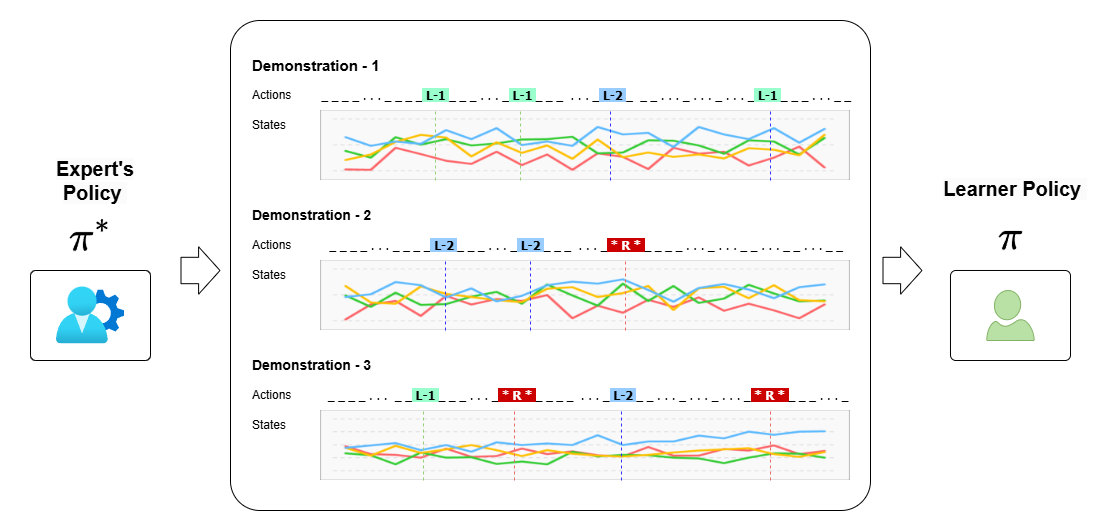
\includegraphics[width=\linewidth]{images/BC_Diagram.png}
\caption{Behavioral Cloning. Demonstrations from Expert include Actions (e.g. maintenance levels L-1, L-2 or Replace tool *R*) and States (from e.g. equipment health readings from sensors)}
\label{fig:BC}
\end{figure}

Having an expert generate a set of demonstrations $\xi \in \mathcal{D}$, Behavioral Cloning approaches determine a policy $\pi$ that imitates the expert. In the simplest form, this can be accomplished through supervised learning techniques \citep{abbeel2004apprenticeship, yue2018imitation}, where the goal is to solve the optimization problem \eqref{eq:BC} i.e. to minimize the difference between the learned policy and expert demonstrations, using a cost or loss function $L$, \citep{stanford-lectures}.  

\begin{equation}\label{eq:BC}
\hat{\pi}^* = \arg\min_{\pi} \sum_{\xi \in \mathcal{D}} \sum_{s \in \xi} L(\pi(s), \pi^*(s)),
\end{equation}
where $L$ is the loss function, $\pi^*(s)$ is the expert's predictive maintenance policy that suggests the maintenance action for the state $s$, and $\hat{\pi}^*$ is the learned, often approximated, policy.

In practice, different loss functions are used depending on the form of the policy: $p$-norms (e.g. Euclidean norm when $p=2$) or $f$-divergences (e.g. KL divergence).

\subsubsection{Practical implications of BC}
The BC algorithm is therefore simple -- at every time-step $t$ it makes the basic assumption that the imitation has been perfect so far, and continues to obediently copy the expert. As is the case for supervised learning, during the optimization step, the algorithm minimizes the deviation compared to expert trajectories and thus minimizes (only) the 1-step error, \citep{yue2018imitation}. As we shall see next, this assumption can cause a drift-off and cause compounding errors, leading to an incorrect learner. We shall also see how it is addressed. 

As depicted in figure \ref{fig:BC}, the learning processes depends solely on the set of demonstrations provided by the expert. It is often difficult for the experts to cover the entire state space, if they do not uniformly sample the state space or provide samples according to convenience.

\begin{figure}[H]
\centering
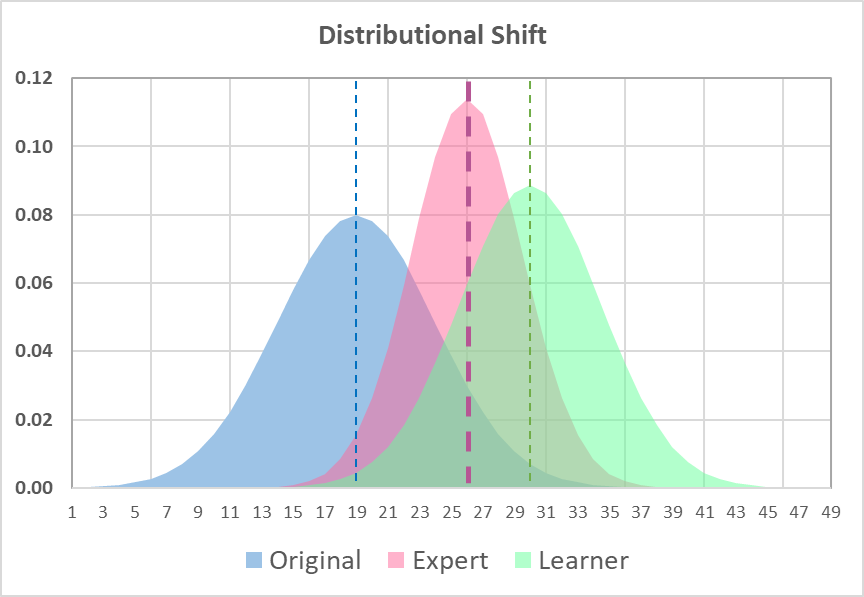
\includegraphics[width=0.6\linewidth]{images/DistributionalShift.png}
\caption{Distributional mismatch (illustrative and exaggerated).}
\label{fig:DistribShift}
\end{figure}

In an industrial maintenance situation this could happen, if for example, the expert picks a certain time of day and a short time period within the entire span of equipment or tool life to provide the demonstrations $\mathcal{D}$.  This will result in a \textit{temporal sequence} of states and actions with a particular distribution. The learned policy will then perform poorly when faced with states not present in $\mathcal{D}$. Behavioral cloning will then \textit{estimate} the policy ${\hat{\pi}}^*$ with its own slightly different distribution of states and these states  that will be visited. The algorithm then begins to drift at every step of learning, leading to compounding errors. This ``distributional shift'', Fig. \ref{fig:DistribShift}, is a major challenge in imitation learning, \citep{yue2018imitation, stanford-lectures}. \textcolor{red}{PLACEMENT -- the importance of randomly sampling and non sequential examples - also PROVIDE DIAGRAM!} 

\cite{Dagger-Ross2010} overcame this core limitation of distributional mismatch in states, by devising the DAgger (Dataset Aggregation) algorithm. It augments existing demonstrations with new expert data when the learned policy ${\hat{\pi}}^*$ leads to states that are not present in the expert dataset $\mathcal{D}$, the expert is queried for more data.

The DAgger algorithm is presented in Algorithm \ref{algo:DAgger}. In the first iteration, the expert's policy is used to gather a dataset $\mathcal{D}$ of trajectories and proceed to train the policy $\hat{\pi}_2$, using supervised learning with an appropriate loss function, that best mimics the expert on those trajectories. It continues this process. Therefore at any iteration $n$, it uses $\hat{\pi}_n$ to gather additional trajectories and append and grown the existing dataset $\mathcal{D}$. The next policy that will be trained, $\hat{\pi}_{n+1}$. will be the policy that best mimics the expert on the entire dataset $\mathcal{D}$.

\noindent \textbf{Notation}:\\
\textbullet\ \quad $\Pi$ is the set of policies the learner is considering and $T$ the time horizon of the task.\\
\textbullet\ \quad Parameter $\beta$ to set how data is obtained from from the expert's behavior. $\beta_i = p^{i-1}$ sets an exponentially decaying probability of using the expert, where $p \in \{0,1, 0.2, ..., 0.9\}$\\

\begin{algorithm}
\onehalfspacing
\caption{DAgger Dataset Aggregation algorithm, \citep{Dagger-Ross2010}}\label{algo:DAgger}
\begin{algorithmic}[1]
	% \State {Data: $\pi^*$}
	% \State {Result: $\hat{\pi}^*$}
	\State {Initialize $\mathcal{D} \leftarrow \emptyset$}
	\State {Initialize $\hat{\pi}_i$}
	\For {i=1 to N}
	\State {$\pi_i = \beta_i \pi^* + (1 - \beta_i) \hat{\pi}_i$}
	\State {Rollout policy $\pi_i$ to sample trajectory $\tau = \{s_0, s_1, ..., s_T\}$ }
	\State {Query expert $\pi^*$ for actions on states provided by $\pi_i$}
	\State {Create dataset $\mathcal{D}_i = \{(s_0, \pi^*(s_0)), (s_1, \pi^*(s_1)), ..., (s_T, \pi^*(s_T))\}$}
	\State {Aggregate datasets: $\mathcal{D} \leftarrow \mathcal{D} \cup \mathcal{D}_i $}
	\State {Retrain policy $\hat{\pi}_{i+1}$ using aggregated dataset $\mathcal{D}$}
	\EndFor
	\State {Return best $\hat{\pi}_i$ on validation}
\end{algorithmic} 
\end{algorithm}

\textcolor{red}{From ROSS: In other words, DAGGER proceeds by collecting a dataset 	at each iteration under the current policy and trains the next 	policy under the aggregate of all collected datasets. The intuition 	behind this algorithm is that over the iterations, we 	are building up the set of inputs that the learned policy is 	likely to encounter during its execution based on previous experience (training iterations).}

\section{Survey of IRL methods for predictive maintenance}\label{sec:SLR}

The field of IL and IRL has been surveyed by researchers. Each of the \textbf{nine} surveys are exhaustive and while some cover the field in general, some are focused on a particular domain. See Table \ref{tbl:Surveys} for details. As of 15-Sep-2024, we see that \textit{none} of the nine surveys cover industrial predictive maintenance. The latest survey \citet{zare2024survey}

And the reason for this is obvious when we search for research on imitation learning applied to predictive maintenance. As seen in Table \ref{tbl:SLR-PdM} and Fig. \ref{fig:SLR}, only 3 artciles come up when we search for IL or IRL applied to PdM. This emphasizes the importance of our survey. 

\begin{figure}[H]
	\begin{floatrow}
		\capbtabbox{%
			\fontfamily{lmss}\selectfont
			\renewcommand{\arraystretch}{1.3}
			\begin{tabular}{L{3cm} R{1cm} R{1.5cm} R{1cm}} 
				\midrule[0.01pt]
				Category & \textbf{Scopus} & \textbf{Web of Science} & \textbf{IEEE Xplore}\\
				\midrule[0.01pt]
				Entire Imitation Learning (IL) field & \textcolor{blue}{4,966}	& 3,516	& 4,679 \\
				IL applied to robotics	& 1,632	& 1,430	& \textcolor{blue}{2,544} \\
				IL applied to autonomous driving & 516	& 322 & \textcolor{blue}{754} \\
				IL applied to predictive maintenance	& \textcolor{blue}{3}	& 1	& 2 \\
				\midrule[0.01pt]
			\end{tabular}
		}{%
			\caption{Research articles by indexing services.\\Data as of 15-Sep-2024.} \label{tbl:SLR}%
		}
		
		\ffigbox{%
			\centering
			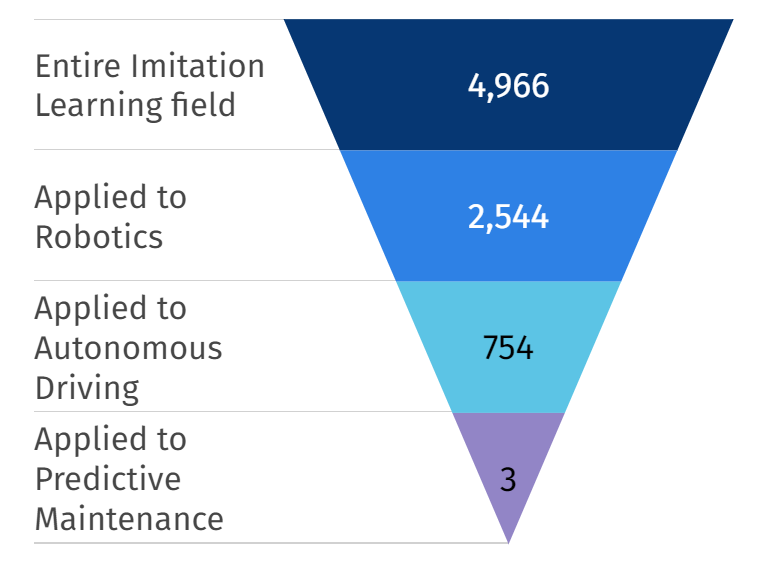
\includegraphics[width=\linewidth]{images/SRL_Articles_funnel.png}
		}{
			\caption{Articles across databases.\\(\textcolor{blue}{Blue} numbers from adjoining Table \ref{tbl:SLR}).}\label{fig:SLR}}
	\end{floatrow}%
\end{figure}

\begingroup
\setlength{\tabcolsep}{6pt}
\begin{table}[h!]
	% \centering
	\renewcommand{\arraystretch}{1.5}
	\fontfamily{lmss}\selectfont
	\begin{tabular}{L{2cm} L{5cm} L{4cm} L{2cm}}
		\midrule[0.01pt]
		\textbf{Category} & \textbf{Focus} & \textbf{Survey articles} & \textbf{Covers PdM?}\\ \midrule[0.01pt]
		Imitation Learning & Autonomous vehicles & \citet{le2022survey} & No\\
		& Robotics, robot arm manipulation & \citet{fang2019survey}, \citet{tai2016survey}, \citet{schaal1999}  & No\\
		& General \par(Covers human computer interaction and computer games in addition to robotics and self-driving cars.) & \citet{zare2024survey}, \citet{hussein2017survey} & No\\
		
		 \midrule[0.005pt]
		Inverse Reinforcement Learning & General & \citet{adams2022survey}, \citet{arora2021survey}, \citet{zhifei2012survey} & No\\
		\midrule[0.01pt]
	\end{tabular}
	\caption{Original surveys covering Imitation Learning and Inverse Reinforcement Learning.} \label{tbl:Surveys}
\end{table}
\endgroup


Search queries:
\begingroup
\setlength{\tabcolsep}{6pt}
\begin{table}[h!]
	% \centering
	\renewcommand{\arraystretch}{2.0}
	\fontfamily{lmss}\selectfont
	\begin{tabular}{L{3cm} L{10cm}}
		\midrule[0.01pt]
		\textbf{Category} & \textbf{Query} \\ \midrule[0.01pt]
		Imitation Learning in general &  \texttt{("Inverse Reinforcement Learning" OR "Imitation Learning" OR "Apprenticeship Learning")} \\
		Application to robotics &  \texttt{("Inverse Reinforcement Learning" OR "Imitation Learning" OR "Apprenticeship Learning") AND ("robot")} \\
		Application to autonomous vehicles &  \texttt{("Inverse Reinforcement Learning" OR "Imitation Learning" OR "Apprenticeship Learning") AND ("autonomous car" OR "autonomous vehicle" OR "autonomous driving" OR "self driving" OR "self-driving")} \\ 
		Application to predictive maintenance &  \texttt{("Inverse Reinforcement Learning" OR "Imitation Learning" OR "Apprenticeship Learning") AND ("predictive maintenance" OR "preventive maintenance" OR "prognostic")} \\ 
		\midrule[0.01pt]
	\end{tabular}
	\caption{Search queries} \label{tbl:SLRQueries}
\end{table}
\endgroup


\subsection{Taxonomy}\label{sec:Taxonomy}

\begin{figure}[H]
	\centering
	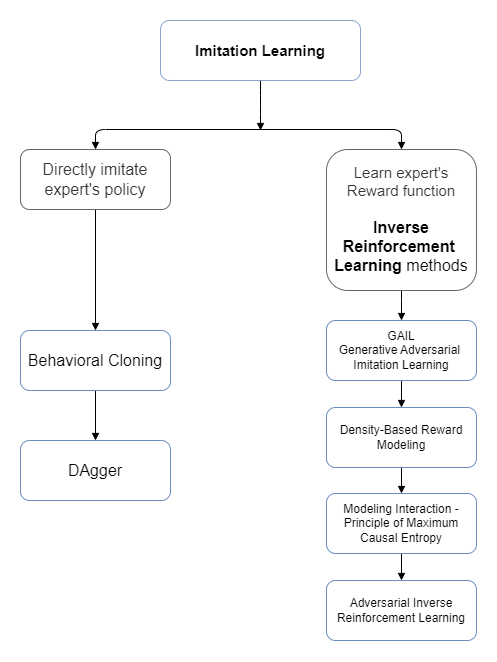
\includegraphics[width=0.4\linewidth]{images/IRL_Taxonomy.png}
	\caption{Taxonomy of Imitation Learning techniques.}
	\label{fig:taxonomy}
\end{figure}

\begingroup
\setlength{\tabcolsep}{6pt}
\begin{table}[h!]
	\centering
	\renewcommand{\arraystretch}{1.5} 
	\begin{tabular}{L{6cm} L{3cm} L{3cm}}
		\midrule[0.01pt]
		& \textbf{Behavioural Cloning} & \textbf{Inverse Reinforcement Learning}\\
		\midrule[0.01pt]
		Direct policy learning & Yes & No \\
		Reward learning & No & Yes \\
		Access to environment & No & Yes \\
		Pre-collected expert demonstrations & Yes & Yes \\
		Need for interactive demonstrator & No & No \\
		\midrule[0.01pt]
	\end{tabular}
	\caption{Types of Imitation Learning, \cite{yue2018imitation}}
	\label{tbl:BC_IRL}
\end{table}
\endgroup



Returned only TWO article: \cite{Chen-2021-Temporal} and \cite{Pinciroli2022-752} 	
\hlc{WordSmith from}: \cite{berant2015imitation} -- To introduce adding the PdM..."To this end, we borrow ideas from imitation learning for structured prediction (xxx). Specifically, we cast agenda-based semantic parsing as a Markov decision process, where the goal is to learn a policy, that given a state (i.e., the current chart and agenda), chooses the best next action (i.e., the parse to pop from the agenda). The supervision signal is used to generate a sequence of"\\
A history $h = (s_1, a_1, . . . , a_T, s_{T+1})$ (\hlc{add a nice Figure! $\rightarrow$ SEE THE COMPRESSED HISTORY section in this article - as it mentions NON sequentioal }) is a sequence of states and actions, such that ... The policy for choosing predictive maintenance actions induces a distribution over histories \\
\begin{equation}
	p_{\theta}(h) = \prod^{T}_{t=1} p_\theta (a_t \mid s_t)    
\end{equation}

\hlc{WordsSmith} ``\textit{This can be accomplished through learning from demonstration, also known as imitation learning. A key principle of imitation learning is that while it may be very difficult to quantify why a certain behavior is desirable, the actual correct behavior is usually known by a human expert. Therefore, rather than having a human expert tune a system to achieve desired behavior, the expert can emonstrate desired behavior and the robot can tune itself to match the demonstration}``

\hlc{\textbf{very important}}: sAMPLED TRajectoriersw  are not sequecntional. why that is ok -- we use the logic in \cite{berant2015imitation} -- compressed history. why it helps: by REMOVING time axis - we remove the logi of replacing after N units of time - i.e. PREVENTIVE maintenance. now it must base it decision on sensor readings - just like calling in an exprt NOT awre of whent the milling tool was installed.

\cite{Chen-2021-Temporal}: Temporal-Logic-Based Semantic Fault Diagnosis With Time-Series Data From Industrial Internet of Things:
The maturity of sensor network technologies has facilitated the emergence of an industrial Internet of Things (IIoT), which has collected an increasing volume of data. Converting these data into actionable intelligence for fault diagnosis is key to reducing unscheduled downtime and performance degradation, among other examples. This article formalizes a problem called semantic fault diagnosis- to construct the formal specifications of faults directly from data collected from IIoT-enabled systems. The specifications are written as signal temporal logic formulas, which can be easily interpreted by humans. To tackle the issue of the combinatorial explosion that arises, we propose an algorithm that combines ideas from agenda-based searching and imitation learning to train a policy that searches formulas in a strategic order. Specifically, we formulate the problem as a Markov decision process, which is further solved with a reinforcement learning algorithm. Our algorithm is applied to time-series data collected from an IIoT-enabled iron-making factory. The results show empirically that our proposed algorithm is both scalable to the size of the data set and interpretable, therefore allowing human users to take actions, for example, predictive maintenance.

\cite{Pinciroli2022-752}: Pinciroli Optimization of the Operation and Maintenance of renewable energy systems by Deep Reinforcement Learning

%Equipment of renewable energy systems are being supported by Prognostics  Health Management (PHM) capabilities to estimate their current health state and predict their Remaining Useful Life (RUL). The PHM health state estimates and RUL predictions can be used for the optimization of the systems Operation and Maintenance (OM). This is an ambitious and challenging task, which requires to consider many factors, including the availability of maintenance crews, the variability of energy demand and production, the influence of the operating conditions on equipment performance and degradation and the long time horizons of renewable energy systems usage. We develop a novel formulation of the OM optimization as a sequential decision problem and we resort to Deep Reinforcement Learning (DRL) to solve it. The proposed solution approach combines proximal policy optimization, imitation learning, for pre-training the learning agent, and a model of the environment which describes the renewable energy system behavior. The solution approach is tested by its application to a wind farm O-and-M problem. The optimal solution found is shown to outperform those provided by other DRL algorithms. Also, the approach does not require to select a-priori a maintenance strategy, but, rather, it discovers the best performing policy by itself



\section{Poiani-2024-Inverse Reinforcement Learning with Sub-optimal Experts}

Inverse Reinforcement Learning Historically,
solving an IRL problem (Adams et al., 2022) involves
determining a reward function that is compatible with
the behavior of an optimal expert. Since the seminal
work of Ng et al. (2000), the problem has been recognized
as ill-posed, as multiple reward functions that
satisfies this requirement exists (Skalse et al., 2023).
For this reason, over the years, several algorithmic
criteria have been introduced to address this ambiguity
issue. These criteria includes maximum margin
(Ratliff et al., 2006), Bayesian approaches (Ramachandran
and Amir, 2007), maximum entropy (Ziebart
et al., 2008), and many others (e.g., Majumdar et al.,
2017; Metelli et al., 2017; Zeng et al., 2022). More
recently, a new line of works have circumvented the
ambiguity issue by redefining the IRL task as the problem
of estimating the entire feasible reward set (Metelli
et al., 2021; Lindner et al., 2022; Metelli et al., 2023).

\href{https://ai.stanford.edu/~ang/papers/icml04-apprentice.pdf}{Apprenticeship Learning via Inverse Reinforcement Learning}

IRL allows one to recover the expert's reward function and then to use this to construct desirable behavior. \citet{ng2000algorithms} suggests that the reward function provides a much more frugal description of behavior. 

Reinforcement learning is founded on the hypothesis that a reward function is a transferable definition of the task, which if rightly defined helps an RL algorithm learn the \textit{policy}. 

\subsubsection{Formal definition}
The inverse reinforcement learning (IRL) problem is formally stated as follows \citep{ng2000algorithms}:

\textbf{Given} 1) measurements of an agent's behavior over time, in a variety of circumstances, 2) if needed, measurements of the sensory inputs to that agent; 3) if available, a model of the environment.

\textbf{Determine} the reward function being optimized

\subsubsection{Algorithm}
\begin{enumerate}
	\item see \citep{sasaki2020} Behavioral cloning from noisy demonstrations - for algo and loss functions
	
	\item  \cite{Pomerleau1991} -- original BC - Pomerleau 1991 Behavioural Cloning
	\item fromt medium article below -- The simplest form of imitation learning is behaviour cloning (BC), which focuses on learning the expert’s policy using supervised learning. An important example of behaviour cloning is ALVINN, a vehicle equipped with sensors, which learned to map the sensor inputs into steering angles and drive autonomously. This project was carried out in 1989 by Dean Pomerleau, and it was also the first application of imitation learning in general.
	
	\item BEHAVIORAL CLONING FROM NOISY DEMONSTRATIONS
	
	\item TORABI - IJCAI 18
	\item also see Stanford article
	\item Simple IRL \href{https://smartlabai.medium.com/a-brief-overview-of-imitation-learning-8a8a75c44a9c}{Medium article}.
	\item DAGGER original \href{https://www.ri.cmu.edu/pub_files/2011/4/Ross-AISTATS11-NoRegret.pdf}{article} and algo
\end{enumerate}

\textcolor{red}{FROM MEDIUM ARTICLE:}\href{https://smartlabai.medium.com/a-brief-overview-of-imitation-learning-8a8a75c44a9c}{smartlabai}.

Behavioural Cloning
The simplest form of imitation learning is behaviour cloning (BC), which focuses on learning the expert’s policy using supervised learning. An important example of behaviour cloning is ALVINN, a vehicle equipped with sensors, which learned to map the sensor inputs into steering angles and drive autonomously. This project was carried out in 1989 by Dean Pomerleau, and it was also the first application of imitation learning in general.

The way behavioural cloning works is quite simple. Given the expert’s demonstrations, we divide these into state-action pairs, we treat these pairs as i.i.d. examples and finally, we apply supervised learning. The loss function can depend on the application. Therefore, the algorithm is the following:

In some applications, behavioural cloning can work excellently. For the majority of the cases, though, behavioural cloning can be quite problematic. The main reason for this is the i.i.d. assumption: while supervised learning assumes that the state-action pairs are distributed i.i.d., in MDP an action in a given state induces the next state, which breaks the previous assumption. This also means, that errors made in different states add up, therefore a mistake made by the agent can easily put it into a state that the expert has never visited and the agent has never trained on. In such states, the behaviour is undefined and this can lead to catastrophic failures.

simple
1. Collect demonstrations (t* trajectories) from expert
2. Treat the demonstrations as i.i.d. state-action pairs: (so, ao), (sj, aj), ...
3. Learn Tte policy using supervised learning by minimizing the loss function
L(a*,To(s))

Still, behavioural cloning can work quite well in certain applications. Its main advantages are its simplicity and efficiency. Suitable applications can be those, where we don’t need long-term planning, the expert’s trajectories can cover the state space, and where committing an error doesn’t lead to fatal consequences. However, we should avoid using BC when any of these characteristics are true.

Direct Policy Learning (via Interactive Demonstrator)
Direct policy learning (DPL) is basically an improved version of behavioural cloning. This iterative method assumes, that we have access to an interactive demonstrator at training time, who we can query. Just like in BC, we collect some demonstrations from the expert, and we apply supervised learning to learn a policy. We roll out this policy in our environment, and we query the expert to evaluate the roll-out trajectory. In this way, we get more training data, which we feedback to supervised learning. This loop continues until we converge.

The way the general DPL algorithm works is the following. First, we start with an initial predictor policy based on the initial expert demonstrations. Then, we execute a loop until we converge. In each iteration, we collect trajectories by rolling out the current policy (which we obtained in the previous iteration) and using these we estimate the state distribution. Then, for every state, we collect feedback from the expert (what would have he done in the same state). Finally, we train a new policy using this feedback.

To make the algorithm work efficiently, it is important to use all the previous training data during the teaching, so that the agent “remembers” all the mistakes it made in the past. There are several algorithms to achieve this, in this article I introduce two them: Data Aggregation and Policy Aggregation. Data aggregation trains the actual policy on all the previous training data. Meanwhile, policy aggregation trains a policy on the training data received on the last iteration and then combines this policy with all the previous policies using geometric blending. In the next iteration, we use this newly obtained, blended policy during the roll-out. Both methods are convergent, in the end, we receive a policy which is not much worse than the expert. More information about these methods can be found here.

The full algorithm is the following:





\section{TO-DO}

1. SLR \\
2. IRL - general concepts and notes \\
3. Taxonomy \\
4. NOTES on BC , other techhniuwues\\
5. Tutorial \\
========== 5.1 environment description\\
========== 5.2 data  description\\
========== flow of tutoria; \\

6. Table of hyper-parms / nw archtecture\\



\clearpage

\section{Approach}

1. \textbf{Tutorial}: Use IEEE Access paper (\href{https://ieeexplore.ieee.org/document/9086464}{see below}) - as basis of writing a Tut paper\\
2. \textbf{IRL}: For solid IRL basics, \textbf{survey}, \textbf{challenges} and \hlc{selecting},  algo. math - see - Saurabh 2020 - A Survey of Inverse Reinforcement Learning: Challenges, Methods and Progress. Also see basic --- Algorithm 1: Template for IRL \\
3. \textbf{IRL in simple terms}: Find better simple language than this --  See "simple" language and \textbf{KEY STEPS AND ALGO.} in (\href{https://thegradient.pub/learning-from-humans-what-is-inverse-reinforcement-learning/}{The Gradient}) \\
4. IRL - AndrewNg article - for IRL basic language and ref. 

\subsection{FIND BETTER SIMPLE language than this =--- }

\textbf{key steps are algorithm are to:}
\begin{itemize}
	\item Estimate the value of our optimal policy for the initial state, as well as the value of every generated policy 	by taking the average cumulative reward of many randomly sampled trials.
	
	\item Generate an estimate of the reward function by solving a linear programming problem. Specifically, set to maximize the difference between our optimal policy and each of the other generated policies.
	
	\item After a large number of iterations, end the algorithm at this step.
	
	\item Otherwise, use a standard RL algorithm to find the optimal policy for. This policy may be different from the given optimal policy, since our estimated reward function is not necessarily identical to the reward function we are searching for.
	
	\item Add the newly generated policy to the set of candidate policies, and repeat the procedure.
\end{itemize}


\section{TUTORIAL PAPER}\label{sec:Tutorial}

\textbf{Refs for tut section:}
\begin{enumerate}
	\item CHAI - \cite{CHAI}
	\item Imitation algos -- \cite{imitation-algos}
\end{enumerate}
\par

IEEE Access tuturial paper -- \href{https://ieeexplore.ieee.org/document/9086464}{A Tutorial and Future Research for Building a Blockchain-Based Secure Communication Scheme for Internet of Intelligent Things} 

2 column x 15 pgs. paper

\textbf{TUTORIAL Elements}:\\
1. Algo of Consensus mech\\
2. pg. 11 Table 3 Simulation params - machine info etc\\
3. pg. 11 E. PRACTICAL DEMONSTRATION - -also contains Java code snippets\\
4. only 2 impacts analye d - imapct of no. users and no. blocks \\
5. computation time for number of users\\






pg. 1. Abstract: "In this paper, we propose a tutorial that aims in desiging a generalized blockchain"\\
pg. 5: Table 1 - Summary of Algos\\
pg. 6: Motivation - "In this tutorial work, we propose a generalized blockchainbased secure communication scheme, mainly from the authentication key management perspective point of view, for IoIT environments."\\\\
pg. 6: "C. MAIN CONTRIBUTIONS":\\\\
The contributions of this paper are listed below.\\
- The impact of blockchain on the existing communication environments is discussed.\\
- The details of different types of blockchain are provided. Some of the famous consensus algorithms are also discussed.\\
- We propose a blockchain-based, secure communication scheme for the Internet of Intelligent Things (IoIT).\\
- The different applications of blockchain-based IoIT communication environments are discussed.\\
- Network and attack models for blockchain-based IoIT communication environments are described, which are helpful in designing a security protocol for such communication environments.\\
- A practical demonstration of the proposed scheme is conducted in order to measure the impact of the proposed scheme on the performance of essential parameters.\\
- Finally, future research challenges in blockchain-based IoIT communication environments are highlighted, which will be helpful to future researchers.\\

\section{WORDS-SMITH}
To this end, we borrow ideas from imitation learning for structured prediction (xxx). Specifically, we cast agenda-based semantic parsing as a Markov decision process, where the goal is to learn a policy, that given a state (i.e., the current chart and agenda), chooses the best next action (i.e., the parse to pop from the agenda). The supervision signal is used to generate a sequence of


\textbf{Paper: Automated Anomaly Detection via Curiosity-Guided Search and Self-Imitation Learning}\\
- Specifically, we first design a curiosity-guided search strategy to overcome the curse of local optimality\\
- A controller, which acts as a search agent, is encouraged to take actions to maximize the information gain about the controller's internal belief.\\
- We further introduce an experience replay mechanism based on self-imitation learning to improve the sample efficiency\\

Reinforcement learning has established itself as an \hlc{transformative force in the realm of xxx, demonstrating their versatility and efficacy across a variety of applications. The ability to model complex data distributions and generate high-quality samples has made xx particularly effective in tasks such as image generation and reinforcement learning. The paper first provides a basic background of GDMs and their applications in network optimization. This is followed by a series of case studies, showcasing the integration of GDMs with Deep Reinforcement Learning (DRL), These case studies underscore the practicality and efficacy of GDMs in real-world scenarios, offering insights into network design. We conclude with a discussion on potential future directions for GDM research and applications, providing major insights into how they can continue to shape the future of network optimization.}


\hlc{The contributions of this paper are summarized as follows:}\\
• We identify a novel and challenging problem (i.e., automated outlier detection) and propose a generic framework AutoOD. To the best of our knowledge, AutoOD describes the first attempt to incorporate AutoML with an outlier detection task, and one of the first to extend AutoML concepts into applications from data mining fields.\\
• We carefully design a search space specifically tailored to the automated outlier detection problem, covering architecture settings, outlier definitions, and the corresponding objective functions.\\
• We propose a curiosity-guided search strategy to overcome the curse of local optimality and stabilize search process\\
• We introduce an experience replay mechanism based on the self-imitation learning to improve the sample efficiency.\\
• We conduct extensive experiments on eight benchmark datasets to demonstrate the effectiveness of AutoOD, and provide insights on how to incorporate AutoOD to the realworld scenarios.\\


\subsection{Citations}

\citep{Tabatabaie2021}: \citefield{Tabatabaie2021}{title}
\cite{Wang2023} \\
\citet{Mao2018-1928}\\
\citep{Wabartha2020-2140}\\

\begingroup
\setlength{\tabcolsep}{6pt}
\begin{table}[h!]
	\centering
	\renewcommand{\arraystretch}{2} 
	
	\begin{tabular}{L{4cm} L{4cm} L{6cm}}	
		\textbf{Article} & \textbf{Application domain} & \textbf{Use-case}\\
		\midrule[0.005pt]
		\citet{Pinciroli2022-752} & Wind farms & Suggest maintenance actions \\
		\citet{Mao2018-1928}, 	 & Wind farms & Suggest maintenance actions \\
		\midrule[0.01pt]
	\end{tabular}
	\caption{Articles using Imitation Learning for predictive maintenance.}
	\label{tbl:SLR-PdM}
\end{table}
\endgroup	


\section{SAMPLE ABSTRACTS}


\subsubsection{Castro Tome - Event-Driven Data Acquisition for Electricity Metering: A Tutorial}
``\hlc{Here, our objective is to provide a comprehensive tutorial of improvements in EDM based on the (algorithmic) definition of the events in a semantic manner, considering also different types of filters and individual definition of thresholds.}``\\ \\

Abstract—This paper provides a tutorial on the most recent advances of event-driven metering (EDM) while indicating potential extensions to improve its performance. We have revisited the effects on signal reconstruction of (i) a fine-tuned procedure for defining power variation events, (ii) consecutive-measurements filtering that refers to the same event, (iii) spike filtering, and (iv) timeout parameter. We have illustrated via extensive numerical results that EDM can provide high-fidelity signal reconstruction while decreasing the overall number of acquired measurements to be transmitted. Its main advantage is to only store samples that are informative based on predetermined events, avoiding redundancy and decreasing the traffic offered to the underlying communication network. This tutorial highlights the key advantages of EDMand points out promising research directions.

Intro $\rightarrow$ II. EVENT-DRIVEN METERING: OVERVIEW $\rightarrow$
\clearpage
\section{Acronyms and notations}
\begin{table}[h]
	\renewcommand\arraystretch{1.5}
	\caption{Notation}
	\begin{tabular}{@{} l L{12cm} @{}}
		$S$&Set of all valid states\\
		$A$&Set of all valid actions\\
		$s_t$&State\\
		$s'$, $s_{(t+1)}$& Next state\\
		$a_t$&Action\\
		$a'$, $a_{(t+1)}$& Next action\\
		$P$, $P(s'\mid s,a)$&Probability distribution of state transitions\\
		$R(t)$&Reward function\\
		$\gamma$ & Discount factor\\
		$\pi_{\theta}$ & Policy $\pi$ with learnable parameters $\theta$\\
		$V^{\pi}(s)$ & Value function\\
		$Q^{\pi}(s, a)$&Action-value function (Q value)\\ \\
		\multicolumn{2}{l}{\textbf{Notations -- \cite{Osa-2018}}}\\\midrule
		$x$ & system state\\
		$s$ & context\\
		$\phi$ & feature vector\\
		$u$ & Predictive maintenance action\\
		$\tau$ & trajectory\\
		$\pi$ & Policy\\
		$\mathcal{D}$ & dataset of demonstrations\\
		$q$ & probability distribution induced by an expert’s policy\\
		$p$ & probability distribution induced by a learner’s policy\\
		$t$ & time\\
		$T$ & finite horizon\\
		$N$ & number of demonstrations\\
		$E$ & superscript representing an expert e.g. $\pi^E$ denotes an expert`s policy\\
		$L$ & superscript representing a learner e.g. $\pi^L$  denotes a learner’s policy\\
		$demo$ & superscript representing a demonstration by an expert $\tau^{demo}$ denotes a trajectory demonstrated by an expert\\
		
	\end{tabular}
\end{table}

\begin{table}[h]
	\renewcommand\arraystretch{1.05}
	\begin{center}
		\begin{minipage}{\textwidth}
			\caption{Acronyms}
			\begin{tabular}{@{} l L{4cm} l L{4cm} @{}}
				\multicolumn{4}{l}{\textbf{Maintenance related terms:}}\\\midrule
				CBM& Condition Based Maintenance&CM & Corrective Maintenance\\
				EoL& End-of-life & KPI&Key Performance Indicator\\
				MIMO&Multiple-input multiple-output & PdM & Predictive Maintenance\\
				PdM& Predictive Maintenance&PHM& Prognostic Health Management\\
				PHM& Prognostic Health Management&PM & Preventive Maintenance\\
				RTFP&Run-to-failure based maintenance policy&RUL& Remaining useful life\\
				SBP& State-based maintenance policy&TBP&Time-based maintenance policy\\ \\
				
				\multicolumn{4}{l}{\textbf{Algorithms:}} \\ \midrule
				CNN&Convoluted Neural Network&LSTM&Long Short Term Memory\\
				A-C& Actor-Critic&PG&Policy Gradient methods\\
				DDPG&Deep Deterministic Policy Gradient&PPO&Proximal Policy Optimization\\
				DQN&Deep Q-Network&DDQN&Double Deep Q-Network\\ \\
				
				\multicolumn{4}{l}{\textbf{Reinforcement Learning:}}\\\midrule
				ML & Machine Learning&RL & Reinforcement Learning\\
				MDP & Markov Decision Process&HM-MDP & Hidden-Mode MDP\\
				POMDP & Partially Observable MDP&SMDP & Semi-MDP\\ \\
				% \botrule
			\end{tabular}
		\end{minipage}
	\end{center}
\end{table}

\clearpage
\printbibliography %Prints bibliography

\end{document}